\documentclass[letterpaper, 12pt]{article}

\usepackage[utf8]{inputenc}
\usepackage[english, spanish]{babel}
\usepackage{fullpage}
\usepackage{graphicx}
\usepackage{amsmath}
\usepackage{enumitem}
\usepackage{chngcntr}
\usepackage{setspace}
\usepackage{url}
\usepackage{csquotes}
\usepackage{float}
\usepackage{verbatim}
\usepackage{tabularx}
\usepackage{amsmath}
\usepackage{caption}
\usepackage{bm}
% \usepackage{hyperref}

\counterwithin{figure}{section}
\renewcommand{\thesection}{\arabic{section}}
\renewcommand{\thesubsection}{\thesection.\arabic{subsection}}
\renewcommand{\baselinestretch}{1.5}
\renewcommand{\thefigure}{\arabic{figure}}

\usepackage[style=numeric, maxnames=6, minnames=3, backend=biber, parentracker=true, sorting=none]{biblatex}
\DefineBibliographyStrings{english}{%chktex-file 1 chktex-file 6
	andothers = {\em et\addabbrvspace al\adddot}
}
\addbibresource{./Bibliography/bibliography.bib}

\usepackage{array}
\usepackage{enumitem}

\setlength{\parskip}{20pt}

\newcommand{\bolditalic}[1]{\textbf{\textit{#1}}}

% chktex-file 24

\begin{document}

\begin{titlepage}
	\centering
	
\includegraphics[width=0.3\textwidth]{Images/logo_utb.png}\par\vspace{1cm}
	{\scshape\LARGE Universidad Tecnológica de Bolívar \par}
	\vspace{1cm}

	{\scshape\Large FÍSICA CALOR Y ONDAS \par}
	\vspace{2.5cm}

	% chktex-file 8
	\slshape {\Large \bfseries{} Avance del proyecto No. II \\}
	\vspace{2cm}

	\slshape {\itshape{} Mauro González, T00067622 \\}
	\slshape {\itshape{} German De Armas Castaño, T00068765 \\}
	\slshape {\itshape{} Angel Vega Rodriguez, T00068186 \\}
	\slshape {\itshape{} Juan Jose Osorio Ariza, T00067316 \\}
	\slshape {\itshape{} Jorge Rueda Salgado, T00068722 \\}
	\vfill
	Revisado Por \\
	Yady Tatiana Solano Correa\\
	{\large \today\par}
\end{titlepage}

% ! --------------------------------------------------------------------------------------------------------------------------------|>
\section*{\textit{Resumen}}

\begin{quote}
	En el vasto universo de la física, pocas cosas son tan omnipresentes
	como las ondas. En el caso de nuestro proyecto, nos enfocamos en
	la lectura de ondas sonoras y su presencia en el mundo cotidiano.
	Para este segundo informe de avance, mostraremos los logros alcanzados
	hasta el momento, plasmando nuestra idea primigenia del proyecto en un
	programa básico. En este programa, se recopilan estas ondas
	sonoras (ya sea a través de canciones, grabaciones, etc.) para
	luego enviarlas a un servidor y ser representadas mediante
	gráficas, mostrando sus propiedades básicas.

	Hemos implementado un tipo de filtro que nos permite
	mostrar únicamente la información que es de nuestro
	interés, desentrañando sus características y propiedades
	fundamentales, tales como el espectro de la onda, el tempo,
	el ritmo y sus coeficientes centrales en las frecuencias
	Mel (MFCC). Todo esto con la idea de que sea aplicable en
	diversos campos, como la música, la medicina o la ciencia
	de datos.
\end{quote}

% ! --------------------------------------------------------------------------------------------------------------------------------|>

\noindent\makebox[\linewidth]{\rule{\linewidth}{0.4pt}}

\bolditalic{Palabras claves}: \textit{Ondas sonoras, ondas electromiográficas,
	ingeniería del sonido, síntesis de sonido, espectro de
	onda.}

\noindent\makebox[\linewidth]{\rule{\linewidth}{0.4pt}}

% ! --------------------------------------------------------------------------------------------------------------------------------|>
\section*{Objetivos}

% + -------------------------------------------------------------------------|>
\subsection*{Objetivo general}

Diseñar una herramienta de lectura de ondas con el
propósito de adquirir, analizar y visualizar los datos
generados por ondas provenientes de distintas fuentes o
fenómenos, contribuyendo así a la comprensión y estudio de
sus características y patrones, que tenga el potencial de
evolucionar hacia una plataforma avanzada en el futuro.

% + -------------------------------------------------------------------------|>
\subsection*{Objetivos específicos}

\begin{itemize}[label=$\triangleright$]
	\item Realizar varias pruebas para garantizar que el programa
	      funcione de manera óptima y sea capaz de manejar una
	      variedad de formatos de audio.

	\item Representar gráficamente las propiedades fundamentales de
	      una onda sonora y su espectrograma.
\end{itemize}

% ! --------------------------------------------------------------------------------------------------------------------------------|>
\section*{Procedimiento experimental}

\begin{enumerate}
	\item Inicio del programa
	\item Pedir al usuario que seleccione un archivo
	      \begin{figure}[H]
		      \begin{center}
			      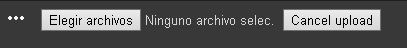
\includegraphics[width=.5\linewidth]{./Images/FileUploadColab.PNG}
			      \caption{}
		      \end{center}
	      \end{figure}

	      Debido a la naturaleza de la herramienta en la que se
	      desarrollo el programa, se abrirá un \textit{Botón} en el
	      que el usuario puede dar click para seleccionar un archivo.

	      \begin{figure}[H]
		      \begin{center}
			      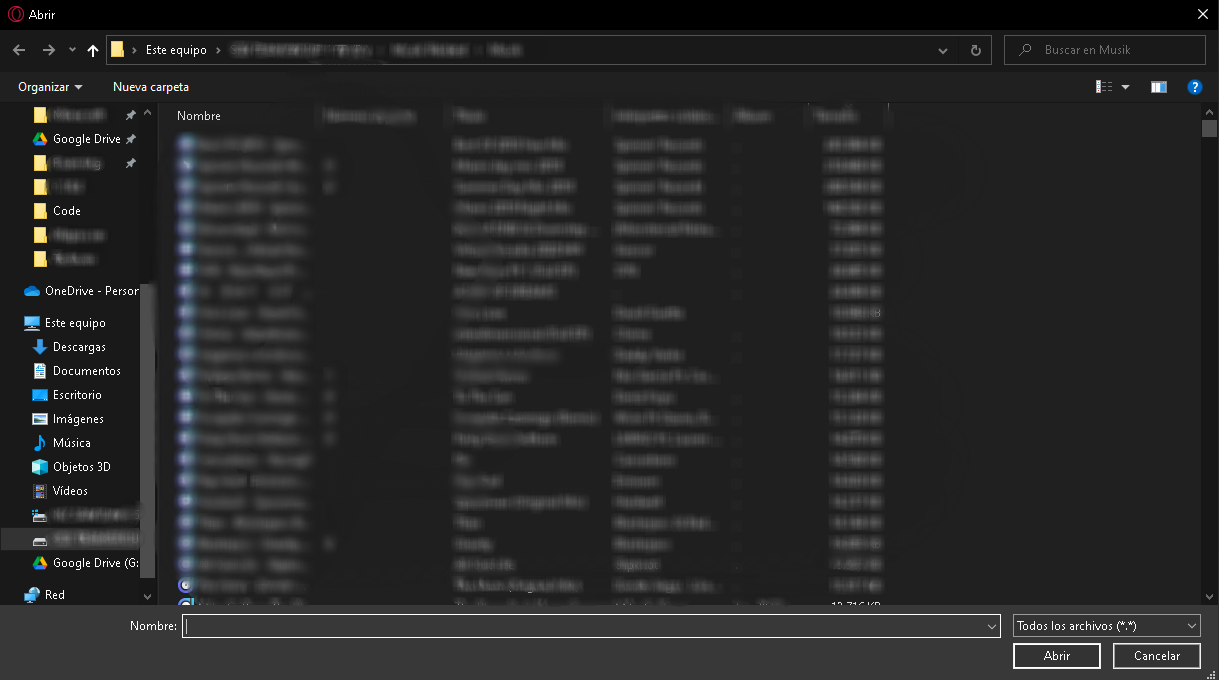
\includegraphics[width=.7\linewidth]{./Images/FileExplorer.png}
			      \caption{}
		      \end{center}
	      \end{figure}

	      Luego, se utiliza el explorador de archivos, para luego
	      proceder con la carga.

	\item Proceder con la carga del archivo a las librerías

	      \begin{figure}[H]
		      \begin{center}
			      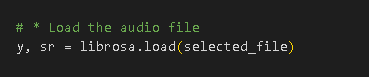
\includegraphics[width=.5\linewidth]{./Images/LoadFile.PNG}
			      \caption{}
		      \end{center}
	      \end{figure}

	      En caso de que el archivo contenga algún error, o
	      directamente no se pueda acceder a él, en ese caso el
	      programa lanzaría una \textit{Exception}, procediendo con
	      la terminación de la ejecución. Caso contrario, se procede
	      con el resto de la ejecución.

	\item Realizar el análisis de audio

	      Luego de verificar que no haya errores en el archivo de
	      audio, se procede a extraer las características que
	      consideremos pertinentes.

	      \begin{figure}
		      \begin{center}
			      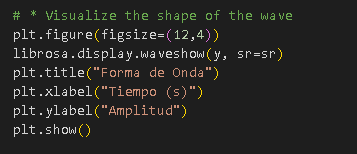
\includegraphics[width=.7\linewidth]{./Images/AudioAnalysisSample_1.PNG}
			      \caption{Bloque de muestra}
		      \end{center}
	      \end{figure}

	      La extracción de características consiste en pequeños
	      bloques, en los que cada uno de estos renderiza la
	      información para ser vista por el usuario.

	      \begin{figure}[H]
		      \begin{center}
			      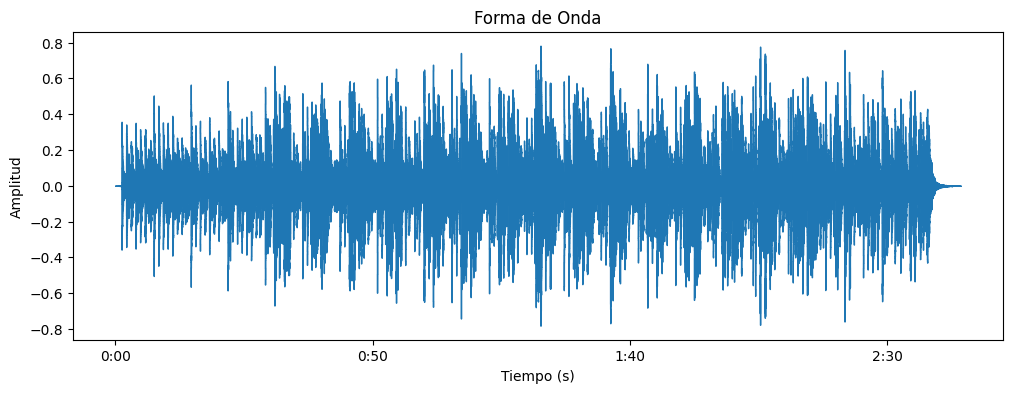
\includegraphics[width=.7\linewidth]{./Images/SampleRunImage_1.png}
			      \caption{}
			      \label{figure:sample_run_image_1}
		      \end{center}
	      \end{figure}

	      La anterior imagen~(\ref{figure:sample_run_image_1}), da un
	      pequeño ejemplo de como seria el \textit{Output final} del
	      programa.
\end{enumerate}

Todo esto se vería resumido en el siguiente flujograma:

\begin{figure}[H]
	\begin{center}
		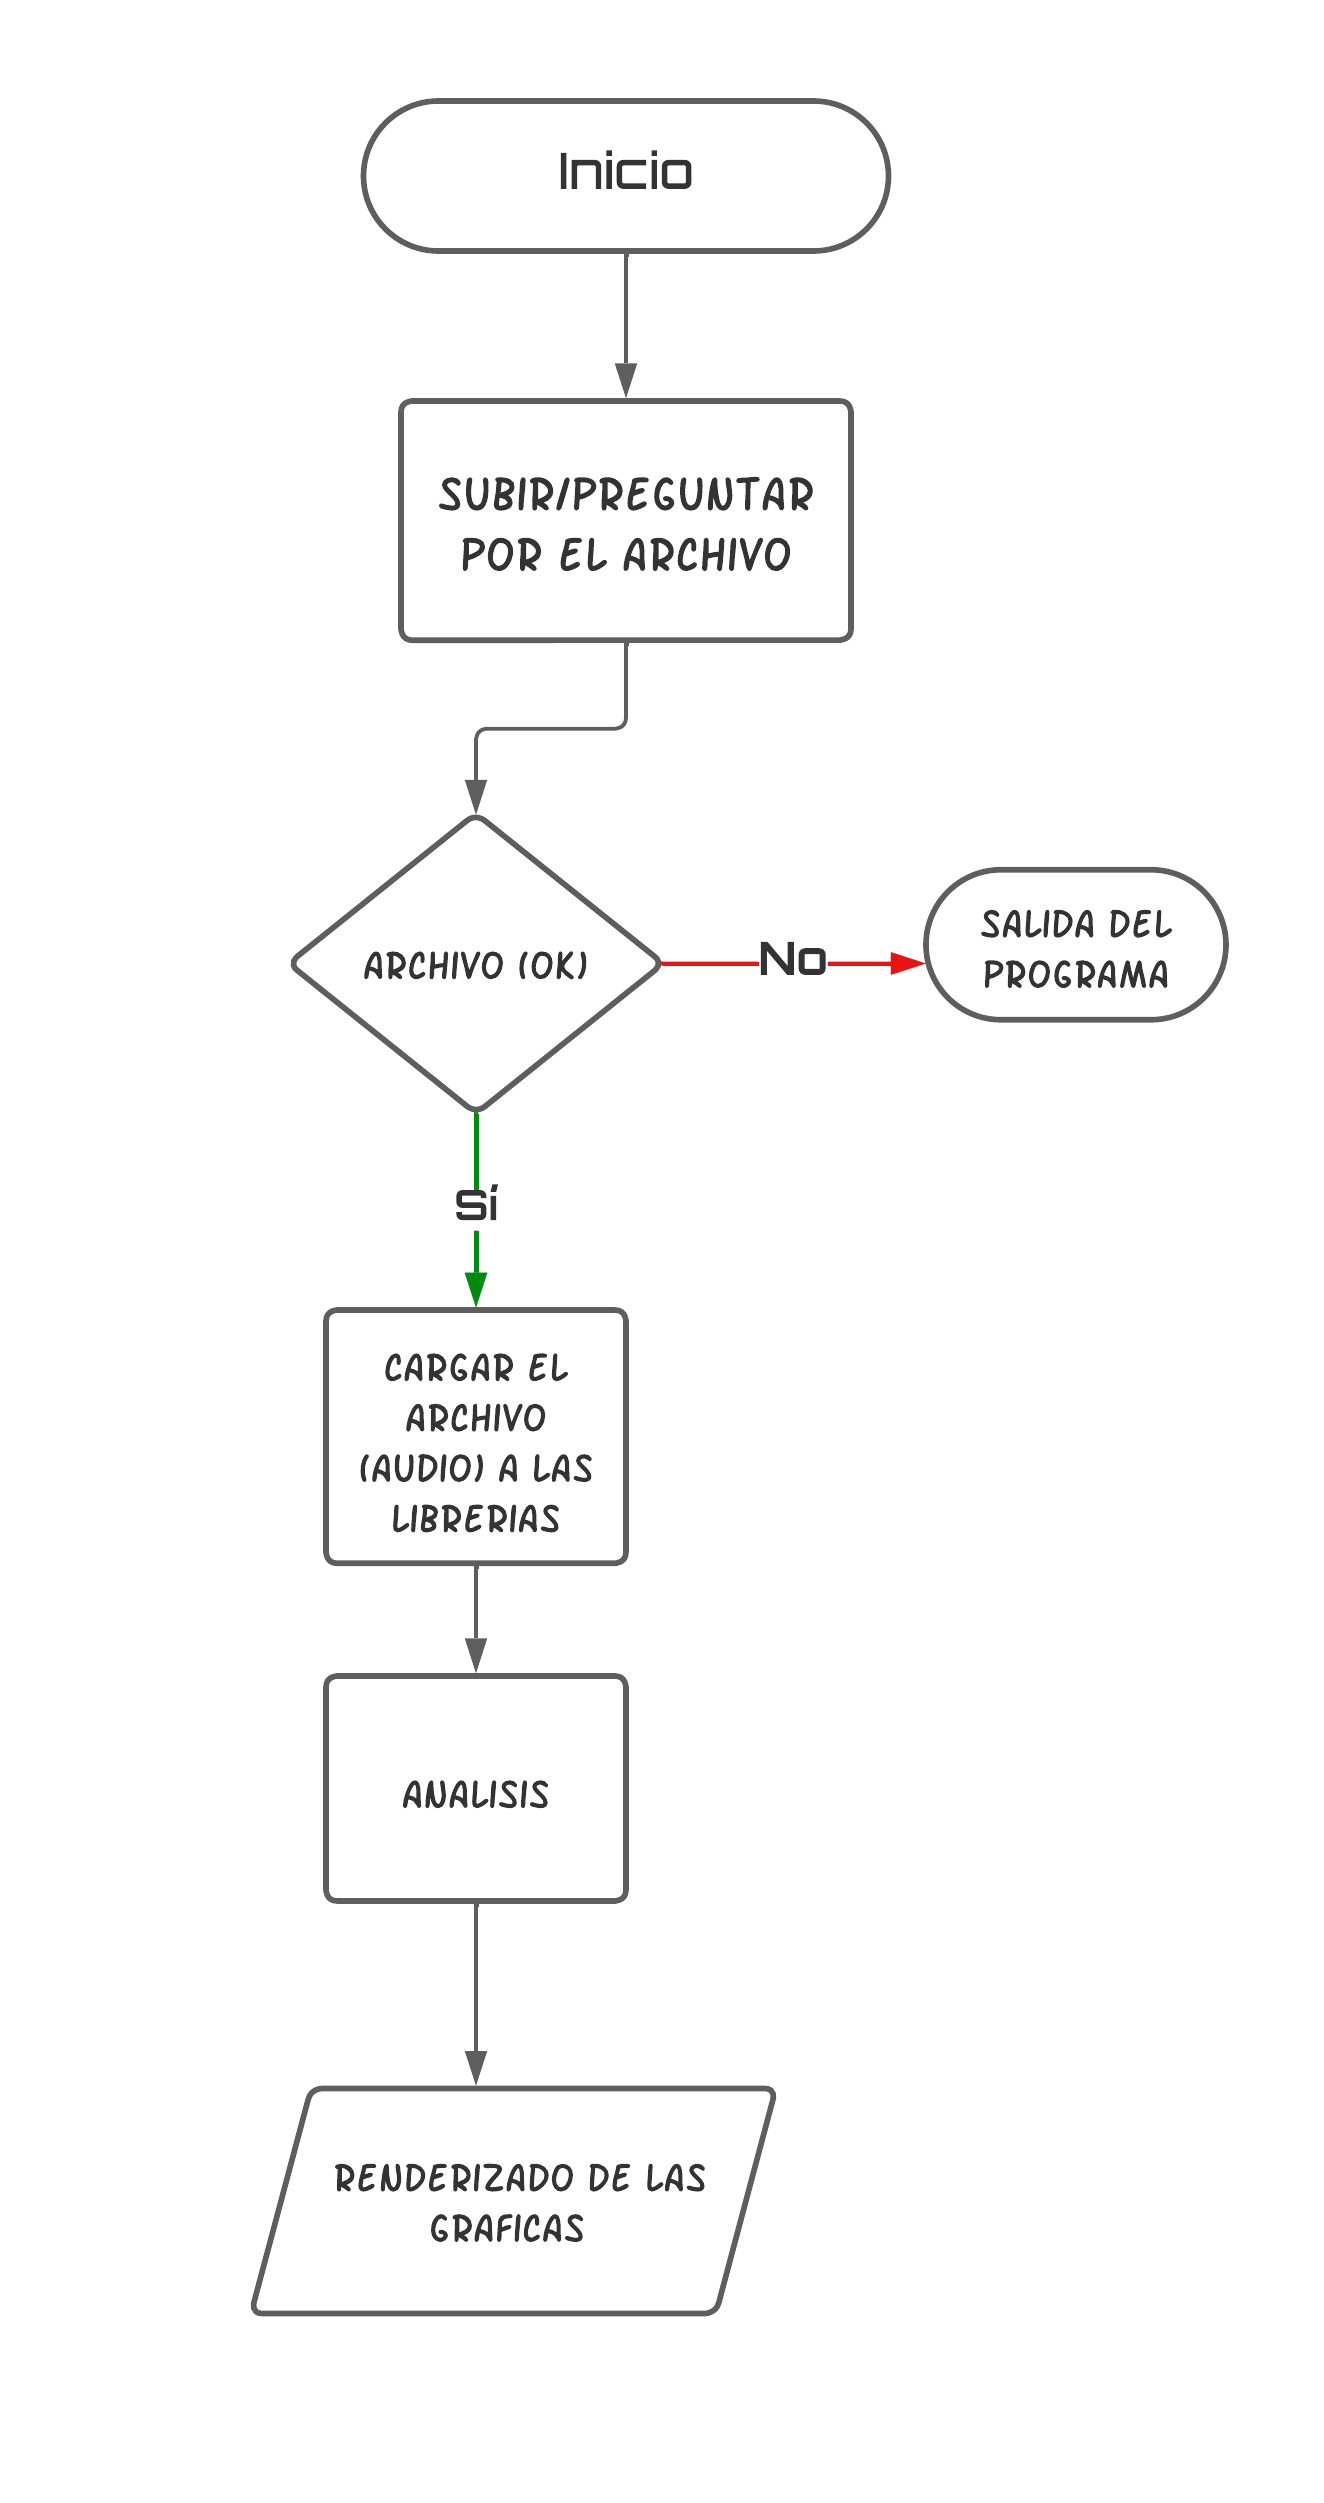
\includegraphics[width=.6\linewidth]{./Images/Flujograma.png}
		\caption{}
	\end{center}
\end{figure}

% ! --------------------------------------------------------------------------------------------------------------------------------|>
\section*{Conclusiones}

En resumen, nuestro proyecto ``Lectura de Ondas'' ha
alcanzado logros significativos desarrollando un programa
capaz de leer y representar de manera óptima el
espectrograma y las propiedades fundamentales de las ondas
sonoras y a la vez abordamos uno de los desafíos
fundamentales: el filtrado de ondas sonoras para extraer
datos relevantes, lo que facilita el análisis preciso de
estas ondas. Estos avances establecen las bases de nuestro
proyecto y nos permite desarrollar y perfeccionar este.

\nocite{source_code}

\printbibliography

\end{document}